\documentclass[a4paper,10pt]{article}

\usepackage[utf8]{inputenc}
\usepackage[english]{babel}
\usepackage[T1]{fontenc}
\usepackage{mathpazo} %http://www.ctan.org/tex-archive/fonts/mathpazo
\usepackage{stmaryrd} %http://www.ctan.org/pkg/stmaryrd
\usepackage{amsmath} %http://www.ctan.org/pkg/amsmath
\usepackage{amssymb}
\usepackage{mathrsfs}
\usepackage[table]{xcolor}% http://ctan.org/pkg/xcolor

\usepackage{amsthm} %http://www.ctan.org/pkg/amsthm
\usepackage{proof}

\usepackage[colorlinks=true]{hyperref} %http://www.ctan.org/tex-archive/macros/latex/contrib/hyperref/
\hypersetup{urlcolor=black,linkcolor=black}

\usepackage{footmisc} %http://www.ctan.org/tex-archive/macros/latex/contrib/footmisc

\usepackage{enumerate}
\usepackage{ulem} %http://www.ctan.org/tex-archive/macros/latex/contrib/ulem
\normalem
\usepackage{cancel} %http://www.ctan.org/tex-archive/macros/latex/contrib/cancel

\usepackage{fullpage} %http://www.ctan.org/tex-archive/macros/latex/contrib/preprint/
\setlength{\parindent}{0pt}
\setlength{\parskip}{\medskipamount}

\usepackage{pgffor}
\usepackage{tikz}
\usetikzlibrary{arrows,shapes.arrows, chains, positioning, automata, graphs}
\usepackage{graphviz}

\usepackage[ruled,vlined,english]{algorithm2e}
\providecommand{\SetAlgoLined}{\SetLine}
\providecommand{\DontPrintSemicolon}{\dontprintsemicolon}

\usepackage{forest}
\usepackage{comment} %http://www.ctan.org/tex-archive/macros/latex/contrib/comment
\usepackage{multirow} %http://www.ctan.org/tex-archive/macros/latex/contrib/multirow
\usepackage{diagbox} %http://www.ctan.org/tex-archive/macros/latex/contrib/diagbox

\usepackage{listings} %http://www.ctan.org/tex-archive/macros/latex/contrib/listings/

\usepackage{textcomp} % arrow, intervals
\usepackage{stmaryrd} % integer intervals

\lstset{numbers=left,language=Caml}

\newcounter{ThComp}
\newcounter{DefComp}

\newtheorem*{fact}{Fact}
\newtheorem*{csq}{Consequence}
\newtheorem{thm}[ThComp]{Theorem}
\newtheorem{theorem}[ThComp]{Theorem}
\newtheorem{propo}[ThComp]{Proposition}
\newtheorem{proposition}[ThComp]{Proposition}
\newtheorem{lemma}[ThComp]{Lemma}
\newtheorem*{corol}{Corollary}
\newtheorem{prop}[ThComp]{Property}
\newtheorem{property}[ThComp]{Property}
\theoremstyle{definition}
\newtheorem*{ex}{Example}
\newtheorem*{exs}{Examples}
\newtheorem{exo}{Exercise}
\newtheorem{question}{\large{Question}}
\newtheorem{defi}[DefComp]{Definition}
\newtheorem*{notation}{Notation}
\newtheorem{definition}[DefComp]{Definition}
\newtheorem{algo}{Algorithm}
\theoremstyle{remark}
\newtheorem*{Rq}{Remark}


\newcommand{\RR}{\mathbb{R}}
\newcommand{\ZZ}{\mathbb{Z}}
\newcommand{\NN}{\mathbb{N}}
\newcommand{\PP}{\mathbb{P}}
\newcommand{\EE}{\mathbb{E}}
\newcommand{\IE}{\mathbb{E}}
\newcommand{\IR}{\mathbb{R}}
\newcommand{\IZ}{\mathbb{Z}}
\newcommand{\IN}{\mathbb{N}}
\newcommand{\IP}{\mathbb{P}}

\newcommand{\cN}{\mathcal{N}}
\newcommand{\cF}{\mathcal{F}}
\newcommand{\ck}{\mathcal{K}}
\newcommand{\cNU}{\mathcal{NU}}
\newcommand{\cL}{\mathcal{L}}
\newcommand{\N}{\mathcal{N}}
\newcommand{\F}{\mathcal{F}}
\renewcommand{\L}{\mathcal{L}}
\newcommand{\A}{\mathcal{A}}

\newcommand{\ens}[1]{\left\{ #1 \right\}}
\newcommand{\set}[1]{\left\{ #1 \right\}}
\renewcommand{\leq}{\leqslant}
\renewcommand{\geq}{\geqslant}
\renewcommand{\le}{\leqslant}
\renewcommand{\ge}{\geqslant}
\newcommand{\cplx}[1]{\mathcal O \left( #1 \right)}
\newcommand{\floor}[1]{\left \lfloor #1 \right \rfloor}
\newcommand{\ceil}[1]{\left\lceil #1 \right\rceil}
\newcommand{\brackets}[1]{\left\llbracket #1 \right\rrbracket}
\newcommand{\donne}{\rightarrow}
\newcommand{\gives}{\rightarrow}
\newcommand{\dans}{\to}
\newcommand{\booleen}{\set{0,1}^*}
\newcommand{\eps}{\varepsilon}
\renewcommand{\implies}{~\Rightarrow~}
\newcommand{\tildarrow}{\rightsquigarrow}
\newcommand{\blank}{\texttt{\char32}}
\newcommand{\trans}[1]{\xrightarrow{#1}}
\newcommand{\rules}[1]{\xrightarrow{#1}}
\newcommand{\todo}[1]{\Large\textcolor{red}{#1}\normalsize}
\newcommand{\argmin}{\text{argmin}}
\newcommand{\rainbowdash}{\vdash}
\newcommand{\notrainbowdash}{\nvdash}
\newcommand{\rainbowDash}{\vDash}
\newcommand{\notrainbowDash}{\nvDash}
\newcommand{\Rainbowdash}{\Vdash}
\newcommand{\notRainbowdash}{\nVdash}
\newcommand{\bottom}{\bot}

%TD/TP
\newenvironment{answer}{\color{blue}}{}

\newcommand{\ddelta}{\delta^{\dag}}
\newcommand{\ddeltat}{\delta^{\dag^t}}
\newcommand{\ddeltatt}{\delta^{\dag^{2t}}}
\newcommand{\xinf}{X^{\infty}}


%#############################################################################################################%
%#############################################################################################################%
%#############################################################################################################%

\title{Distributing the Heat Equation}
\author{Tom Cornebize \and Yassine Hamoudi}
\date{December 7th, 2014}

\begin{document}

\maketitle

%#############################################################################################################%
%#############################################################################################################%
%#############################################################################################################%

\section{Cellular automata}

%#############################################################################################################%

\subsection*{Question 1}

\begin{lemma}
  \label{nextStep}
  $N^2$ applications of function $\delta$ are necessary to compute $X^t$ from $X^{t-1}$.
\end{lemma}

\begin{proof}
 Each cell $X^{t}_{i,j}$ needs one application of $\delta$ to be computed from $X^{t-1}_{i,j}$. There are $N^2$ cells, so $N^2$ applications of $\delta$ are needed.
\end{proof}

\begin{prop}
  $tN^2$ applications of function $\delta$ are necessary to compute $X^t$ on \textlbrackdbl $0,N-1$ \textrbrackdbl$^2$.
\end{prop}

\begin{proof}
 $X^t$ is obtained after $t$ applications of $\ddelta$ on $X^0$. Each application needs $N^2$ calls to $\delta$ according to lemma \ref{nextStep}. The whole computation needs $tN^2$ applications of $\delta$.
\end{proof}

%#############################################################################################################%

\subsection*{Question 2}

Let $p^2$ be the number of processors.

For the sake of simplicity, \underline{we will assume throughout the homework} that $p$ divides $N$. Take $n = \frac{N}{p}$.

We divide the grid into square zones of size $n$. Each of this zones is given to one processor, which stores the data in its own memory and performs the computation of $\delta$ for all its cells. See figure \ref{q2:draw} for an example.

At each step of computation, each processor updates its sub-matrix cells using a temporary sub-matrix that replaces the old one once the computation step is finished. Indeed,  if we update the cells ``in place'', we overwrite values that are still necessary to compute other cells.

The computation of $\delta$ for the cells at the edges of the zones requires communication to retrieve the current states of their neighbours in other zones.

\begin{figure}
\caption{Graphical representation of the topology for $N=6$ and $p^2=9$.}
\label{q2:draw}
\begin{center}
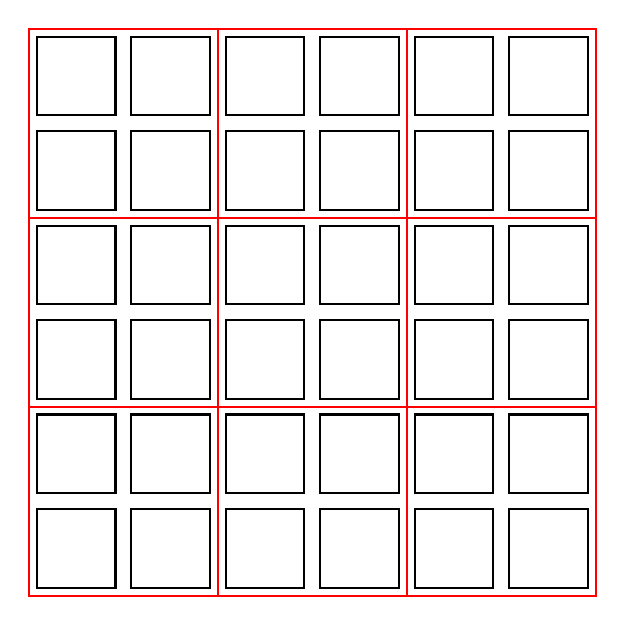
\begin{tikzpicture}
    \tikzstyle{case}=[draw, minimum height=1cm, minimum width=1cm, thick, fill=white, anchor=south west];
    \tikzstyle{redcase}=[draw, minimum height=2.4cm, minimum width=2.4cm, thick, fill=none, draw=red, anchor=south west];

    \foreach \x in {0,...,5} {
        \foreach \y in {0,...,5} {
            \node[case] at (1.2*\y,1.2*\x) {};
        }
    }
    \foreach \x in {0,...,2} {
        \foreach \y in {0,...,2} {
            \node[redcase] at (2.4*\y-0.1,2.4*\x-0.1) {};
        }
    }
\end{tikzpicture}
\end{center}
\end{figure}

%#############################################################################################################%

\subsection*{Question 3}

We assume that $X^t$ is already distributed. Each processor is responsible for a submatrix of $X^t$ of size $n \cdot n$. In practice, each processor also stores the 2 neighbours rows and the 2 neighbours colones of its submatrix. For each processor, we denote by $PREV$ the submatrix of size $(n+2) \times (n+2)$ it stores.

We also assume that the order of messages is preserved.

Let $$\delta(PREV,i,j) = \delta \left( \begin{array}{ | c | c | c |} \hline

  PREV[i-1,j-1] & PREV[i-1,j] & PREV[i-1,j+1] \\ \hline

  PREV[i,j-1] & PREV[i,j] & PREV[i+1,j+1] \\ \hline

  PREV[i+1,j-1] & PREV[i+1,j] & PREV[i+1,j+1] \\ \hline

 \end{array} \right)$$

We consider function \texttt{Send\_X} (resp. \texttt{Receive\_X}) for \texttt{X = Up, Down, Left, Right} which sends (resp. receives) to (resp. from) the corresponding processor. 
We suppose that this function has a time cost of $1$ and a communication cost of $L+b$ where $L$ is the latency and $b$ the bandwidth.

We also consider functions to send an entire row (resp. column) as one single message, to decrease the overall latency. For instance, \texttt{Send\_Down\_Row(n,PREV)} will send to the down processor the $\text{n}^{th}$ row, whereas \texttt{Send\_Up\_Row(0,PREV)} will receive from the up processor a row, which will be stored as the $\text{0}^{th}$ row.
We suppose that this function has a time cost of $n$ and a communication cost of $L+nb$ where $L$ is the latency, $b$ the bandwidth, and $n$ the size of the row/column.

\begin{algorithm}[H]
    \SetKwFunction{sndup}{Send\_Up}
    \SetKwFunction{snddown}{Send\_Down}
    \SetKwFunction{sndleft}{Send\_Left}
    \SetKwFunction{sndright}{Send\_Right}
    \SetKwFunction{rcvup}{Receive\_Up}
    \SetKwFunction{rcvdown}{Receive\_Down}
    \SetKwFunction{rcvleft}{Receive\_Left}
    \SetKwFunction{rcvright}{Receive\_Right}
    \SetKwFunction{sndupr}{Send\_Up\_Row}
    \SetKwFunction{snddownr}{Send\_Down\_Row}
    \SetKwFunction{sndleftc}{Send\_Left\_Column}
    \SetKwFunction{sndrightc}{Send\_Right\_Column}
    \SetKwFunction{rcvupr}{Receive\_Up\_Row}
    \SetKwFunction{rcvdownr}{Receive\_Down\_Row}
    \SetKwFunction{rcvleftc}{Receive\_Left\_Column}
    \SetKwFunction{rcvrightc}{Receive\_Right\_Column}
    \DontPrintSemicolon
    \LinesNotNumbered
        \KwIn{PREV: array[0..n+1,0..n+1] of real}
        \KwOut{NEXT: array[0..n+1,0..n+1] of real}
            \tcc{Columns and row}
                \sndleftc{1,PREV}\;
                \sndrightc{n,PREV}\;
                \sndupr{1,PREV}\;
                \snddownr{n,PREV}\;
                \rcvleftc{0,PREV}\;
                \rcvrightc{n+1,PREV}\;
                \rcvupr{0,PREV}\;
                \rcvdownr{n+1,PREV}\;
            \tcc{Corners}
                \sndup{PREV[1][0]}\;
                \sndup{PREV[1][n+1]}\;
                \snddown{PREV[n][0]}\;
                \snddown{PREV[n][n+1]}\;
                \rcvup{PREV[0][0]}\;
                \rcvup{PREV[0][n+1]}\;
                \rcvdown{PREV[n+1][0]}\;
                \rcvdown{PREV[n+1][n+1]}\;
            \tcc{Computation of $\delta$}
                \For{i=1 \textbf{to} n}{
                    \For{j=1 \textbf{to} n}{
                        $NEXT[i][j] = \delta(PREV,i,j)$\;
                    }
                }
\caption{Iteration on arbitrary automaton\label{algoq3}}
\end{algorithm}

\underline{Time complexity}
\begin{itemize}
 \item \textit{Each processor:} $8(n+1) + n^2 \text{cost}(\delta) = 8(\frac{N}{p}+1) + \left(\frac{N}{p}\right)^2 \text{cost}(\delta) = \cplx{\left(\frac{N}{p}\right)^2}$ if $\text{cost}(\delta) = \cplx{1}$.
 \item \textit{All processors:} $\cplx{N^2}$
\end{itemize}

\underline{Communication complexity}
\begin{itemize}
 \item \textit{Each processor:} $8(L+nb+L+1) = 8(2L+\frac{N}{p}b+1)$.
 \item \textit{All processors:} $8p^2(2L+\frac{N}{p}b+1) = 8(2p^2L+Npb+p^2)$.
\end{itemize}

\textbf{\large{Non-toric grid}}

On a non-toric grid, processors placed on edges cannot send directly their information to their neighbours. They have to pass their messages throughout the whole grid. It needs $p$ steps of communication instead of one.

\underline{Time complexity}
\begin{itemize}
 \item \textit{Each processor on an edge and not on a corner of the grid:} $(6+2p)(8(n+1) + n^2 \text{cost}(\delta))$.
 \item \textit{Each processor on a corner:} $(4+4p)(8(n+1) + n^2 \text{cost}(\delta))$.
 \item \textit{Each processor not on an edge:} $8(n+1) + n^2 \text{cost}(\delta)$.
 \item \textit{All processors:} $4(p-2)(6+2p)(8(n+1) + n^2 \text{cost}(\delta)) + 4(4+4p)(8(n+1) + n^2 \text{cost}(\delta)) + (p-1)^2 (8(n+1) + n^2 \text{cost}(\delta)) = \cplx{N^2}$
\end{itemize}

\underline{Communication complexity}
\begin{itemize}
 \item \textit{Each processor on an edge and not on a corner of the grid:} $6(L+nb+L+1) + 2p(L+nb+L+1) = (6+2p)(2L+\frac{N}{p}b+1)$.
 \item \textit{Each processor on a corner:} $4(L+nb+L+1) + 4p(L+nb+L+1) = (4+4p)(2L+\frac{N}{p}b+1)$.
 \item \textit{Each processor not on an edge:} $8(L+nb+L+1) = 8(2L+\frac{N}{p}b+1)$.
 \item \textit{All processors:} $4(p-2)(6+2p)(2L+\frac{N}{p}b+1) + 4(4+4p)(2L+\frac{N}{p}b+1) + (p-1)^2 8(2L+\frac{N}{p}b+1) = \cplx{p^2 (L + \frac{N}{p}b)}$
\end{itemize}

\textbf{\large{Ring topology}}

On a ring topology we distribute the matrix in a different way. Each processor stores $\frac{N}{p^2}$ contiguous lines of the matrix. Thus, each processor only needs to get/send values to its 2 immediate neighbours in the ring.

\underline{Time complexity}
\begin{itemize}
 \item \textit{Each processor:} $4n + N \cdot \frac{N}{p^2} \text{cost}(\delta)$ (4 rows are exchanged and $N \cdot \frac{N}{p^2}$ cells are updated).
 \item \textit{All processors:} $p^2 (4n + N \cdot \frac{N}{p^2} \text{cost}(\delta))$
\end{itemize}

\underline{Communication complexity}
\begin{itemize}
 \item \textit{Each processor:} $4N(L+nb)$ (each processor sends 2 rows and receive 2 rows).
 \item \textit{All processors:} $p^2 4N(L+nb)$
\end{itemize}

%#############################################################################################################%
%#############################################################################################################%

\section{Average automata}

%#############################################################################################################%

\subsection*{Question 4}
 
 See the implementation in file \texttt{average.c}.
  
%#############################################################################################################%

\subsection*{Question 5}
 
\begin{prop}
 In the case of a \textit{p-average automaton}, $\ddelta$ is linear.
\end{prop}

\begin{proof}
 Let $\ddelta$ be the global transition function of a \textit{p-average automaton}. To prove that $\ddelta$ is linear, it suffices to prove that the local transition function $\delta$ is linear:
 
 \[ \delta \left( \begin{array}{ | c | c | c |} \hline
  a & b & c \\ \hline
  d & e & f \\ \hline
  g & h & i \\ \hline
 \end{array} \right) = (1-p) \cdot e+p \cdot \frac{b+d+f+h}{4}\]
 
 Let consider a real $k \in \RR$ and two local configurations $\begin{array}{ | c | c | c |} \hline
  a & b & c \\ \hline
  d & e & f \\ \hline
  g & h & i \\ \hline
 \end{array}$ and $\begin{array}{ | c | c | c |} \hline
  a' & b' & c' \\ \hline
  d' & e' & f' \\ \hline
  g' & h' & i' \\ \hline
 \end{array}$. We have:
 
 \[\begin{split}
 \delta \left( k \cdot \begin{array}{ | c | c | c |} \hline
  a & b & c \\ \hline
  d & e & f \\ \hline
  g & h & i \\ \hline
 \end{array} + \begin{array}{ | c | c | c |} \hline
  a' & b' & c' \\ \hline
  d' & e' & f' \\ \hline
  g' & h' & i' \\ \hline
 \end{array} \right) & = (1-p) \cdot (k \cdot e+e') + p \cdot \frac{(k \cdot b+b')+(k \cdot d+d')+(k \cdot f+f')+(k \cdot h+h')}{4}  \\
		     & = k \cdot \left( (1-p) \cdot e+p \cdot \frac{b+d+f+h}{4} \right) + (1-p) \cdot e'+p \cdot \frac{b'+d'+f'+h'}{4} \\
		     & = k \cdot \delta \left( \begin{array}{ | c | c | c |} \hline
  a & b & c \\ \hline
  d & e & f \\ \hline
  g & h & i \\ \hline
 \end{array} \right) + \delta \left( \begin{array}{ | c | c | c |} \hline
  a' & b' & c' \\ \hline
  d' & e' & f' \\ \hline
  g' & h' & i' \\ \hline
 \end{array} \right)      
 \end{split}\]
 
Thus $\delta$ is linear, and $\ddelta$ too.
\end{proof}

%%%%%%%%%%%%%%%%%%%%%%%%%%%ù

\begin{defi}
 For $0 \leq i,j \leq N-1$ we define the matrix $E^{i,j}$ such that $E^{i,j}_{i,j} = 1$ and $E^{i,j}_{k,l} = 0$ otherwise.
\end{defi}

\begin{lemma}
 For all $0 \leq i, j, k, l \leq N-1$, $\ddeltat(E^{i,j})_{k,l} = \ddeltat(E^{0,0})_{k-i,l-j}$ (indices are taken modulo $N$). Thus, knowing $\ddeltat(E^{0,0})$ we obtain $\ddeltat(E^{i,j})$ in constant time.
\end{lemma}

Now let's consider a configuration $X$. We have : $X = \sum_{i=0}^{N-1} \sum_{j=0}^{N-1} X_{i,j} \cdot E^{i,j}$. Since $\ddelta$ is linear, for all t : 
\[ \ddeltat (X) = \sum_{i=0}^{N-1} \sum_{j=0}^{N-1} X_{i,j} \cdot \ddeltat (E^{i,j})\]
 
Moreover : 
\begin{equation}
 \label{expanddelta}
 \begin{split}
    \ddeltatt (X) & = \sum_{i=0}^{N-1} \sum_{j=0}^{N-1} X_{i,j} \cdot \ddeltatt (E^{i,j}) \\
		  & = \sum_{i=0}^{N-1} \sum_{j=0}^{N-1} X_{i,j} \cdot \ddeltat(\ddeltat (E^{i,j})) \\
		  & = \sum_{i=0}^{N-1} \sum_{j=0}^{N-1} X_{i,j} \sum_{k=0}^{N-1} \sum_{l=0}^{N-1} \ddeltat (E^{i,j})_{k,l} \cdot \ddeltat (E^{k,l}) \\
		  & = \sum_{i=0}^{N-1} \sum_{j=0}^{N-1} X_{i,j} \sum_{k=0}^{N-1} \sum_{l=0}^{N-1} \ddeltat (E^{0,0})_{k-i,l-j} \cdot \ddeltat (E^{k,l})
 \end{split}
\end{equation}

Thus, for all $0 \leq m, n \leq N-1$:
\begin{equation}
 \label{aveq}
 \begin{split}
    \ddeltatt (X)_{m,n} & = \sum_{i=0}^{N-1} \sum_{j=0}^{N-1} X_{i,j} \sum_{k=0}^{N-1} \sum_{l=0}^{N-1} \ddeltat (E^{0,0})_{k-i,l-j} \cdot \ddeltat (E^{k,l})_{m,n} \\
                        & = \sum_{i=0}^{N-1} \sum_{j=0}^{N-1} X_{i,j} \sum_{k=0}^{N-1} \sum_{l=0}^{N-1} \ddeltat (E^{0,0})_{k-i,l-j} \cdot \ddeltat (E^{0,0})_{m-k,n-l}
 \end{split}
\end{equation}

Especially, for $X = E^{0,0}$:
\begin{equation}
 \label{avequnit}
 \begin{split}
    \ddeltatt (E^{0,0})_{m,n} & = \sum_{k=0}^{N-1} \sum_{l=0}^{N-1} \ddeltat (E^{0,0})_{k,l} \cdot \ddeltat (E^{0,0})_{m-k,n-l}
 \end{split}
\end{equation}

\begin{prop}
 Equations \ref{aveq} and \ref{avequnit} enable us to compute $\ddeltat(X)$ in time $\cplx{\log(t)}$ for a fixed $N$.
\end{prop}

\begin{proof}
For computing $\ddeltatt(X)$ we need to compute $\ddeltat(E^{0,0})$ using equation \ref{avequnit} and then apply equation \ref{aveq} to get $\ddeltatt(X)$. The algorithm is:

\begin{algorithm}[H]
    \DontPrintSemicolon
    \LinesNotNumbered
    \KwIn{t, X}
    \KwOut{$\ddeltat(X)$}
        $R \leftarrow E^{0,0}$; \\
        \For{i=1 \textbf{to} $\log(t) - 1$}{
            Compute $R \leftarrow \delta^{\dag^{2^i}}(E^{0,0})$ using $\delta^{\dag^{2^{i-1}}}(E^{0,0})$ (previous value of $R$) and equation \ref{avequnit}
        }
        Compute and return $\ddeltat(X)$ using $R = \delta^{\dag^{t/2}}(E^{0,0})$ and equation \ref{aveq}
\caption{Iteration on average automaton\label{algoq5}}
\end{algorithm}

 Let $T'(t)$ be the time needed to compute $\ddeltat(E^{0,0})$. According to equation \ref{avequnit} we have:
 \[\begin{split}
    T'(t) & = T'(t/2) + \cplx{1}\\
         & = \cplx{\log(t)}
   \end{split}
\]
 
 Now let $T(t)$ be the time needed to compute $\ddeltat(X)$. According to equation \ref{aveq} and previous remarks, we have:
 \[\begin{split}
    T(t) & = T'(t/2) + \cplx{1} \\
    & = \cplx{\log(t)}
   \end{split}
\]
 
 Thus, applying the operations described in equations \ref{aveq} and \ref{avequnit}, we can compute $\ddeltat(X)$ in time $\cplx{\log(t)}$. 
\end{proof}

\begin{prop}
 The time complexity $T_r(t,N)$ in terms of both $t$ and $N$ is $T_r(t,N) = \cplx{N^4 \cdot \log(t) + N^6}$.
\end{prop}

\begin{proof}
  Let $T_e(t,N)$ be the time needed to compute $\ddeltat(E^{0,0})$. According to equation \ref{avequnit} we have:
 \[\begin{split}
    T_e(t) & = T_e(t/2) + N^2 \cdot N^2 \text{ (there are } N^2 \text{ cells and each one needs to perform } N^2 \text{ sums)} \\
         & = \cplx{N^4 \cdot \log(t)}
   \end{split}
\]  
  
  According to equation \ref{aveq} and the previous algorithm, knowing $\delta^{\dag^{t/2}}(E^{0,0})$ it remains to perform for each cell the four sums described in equation \ref{aveq} (it takes time $\cplx{N^4}$ per cell). Finally, we have:
  \[ T_r(t,N) = T_e(t/2,N) + N^2 \cdot N^4\]
  
  Thus: $T_r(t,N) = \cplx{N^4 \cdot \log(t) + N^6}$.
  
  According to question 3, the complexity in general case is $\cplx{N^2 \cdot t}$. The algorithm using the linearity of $\ddelta$ is more interesting when the number of steps $t$ increases.
\end{proof}

\begin{prop}
 The space complexity $T_s(t,N)$ in terms of both $t$ and $N$ is $T_s(t,N) = \cplx{N^2}$.
\end{prop}

\begin{proof}
 We need $N^2$ space to store the initial matrix.

 When we compute $\delta^{\dag^{2^i}}(E^{0,0})$ using $\delta^{\dag^{2^{i-1}}}(E^{0,0})$, we need to use $N^2$ space to store $\delta^{\dag^{2^i}}$. However, the space used by $\delta^{\dag^{2^{i-1}}}$ can be re-use to compute $\delta^{\dag^{2^{i+1}}}$. Thus, all the computation can be done using $\cplx{N^2}$ space.
 
 The space complexity is the same than in the general case.
\end{proof}

%#############################################################################################################%

\subsection*{Question 6}

Matrices $R$ and $\ddeltat(X)$ are distributed in the same way than in question 2 (each processor stores a submatrix of size $n \cdot n$).

Each step of the \texttt{for} loop of algorithm \ref{algoq5} is performed in the following way:
\begin{itemize}
 \item each processor broadcasts its submatrix to all the other processors.
 \item using equation \ref{avequnit}, each processor updates a temporary submatrix $B$ initially null, as soon as it receives the submatrices it needs.
 \item each processor replaces the part of $R$ it stores by the submatrix $B$.
\end{itemize}

At the end of the previous steps, $\delta^{\dag^{t/2}}(E^{0,0})$ is computed and distributed. $\ddeltat(X)$ is computed in the same way than $\delta^{\dag^{t/2}}(E^{0,0})$ (each processor broadcasts the parts of $X^0$ and $\delta^{\dag^{t/2}}(E^{0,0})$ it stores, the computation is done using equation \ref{aveq}).

\begin{prop}
 The time complexity is $T_t(t,N) = \cplx{\log(t) \cdot N^4 + N^6}$ (we do not count communication time).
\end{prop}

\begin{proof}
 We recall that $n = \frac{N}{p}$.
 
  At each step of the \texttt{for} loop, each processor performs $\cplx{n^2 \cdot N^2}$ operations according to equation \ref{avequnit}. The final computation of $\ddeltat(X)$ using $\delta^{\dag^{t/2}}(E^{0,0})$ needs $\cplx{N^2 \cdot N^4}$ operations. Thus $T_t(t,N) = \log(t) \cdot p^2 \cdot n^2 \cdot N^2 + N^6) = \cplx{\log(t) \cdot N^4 + N^6}$.
\end{proof}

\begin{prop}
 The space complexity is $T_s(t,N) = \cplx{N^2}$.
\end{prop}

\begin{proof}
 Each processor stores 3 arrays of size $n^2$ and needs $\cplx{n^2}$ extra space during broadcast operations. Moreover, this space can be reused at each new step. Thus:
  \[
    \begin{split}
        T_s(t,N) & = \cplx{p^2 \cdot n^2}\\
                 & = \cplx{N^2}
    \end{split}
 \] 
\end{proof}

\begin{prop}
 The communication time complexity is $T_c(t,N) = \cplx{c \cdot p^2 \cdot \log(t) \cdot N^2}$.
\end{prop}

\begin{proof}
 At each step of the \texttt{for} loop, each processor performs $\cplx{p^2}$ broadcasts of a matrix of size $n^2$. Thus:
  \[
    \begin{split}
        T_c(t,N) & = \cplx{c \cdot p^2 \cdot p^2 \cdot \log(t) \cdot n^2} \\
                 & = \cplx{c \cdot p^2 \cdot \log(t) \cdot N^2}
    \end{split}
 \] 
\end{proof}

%#############################################################################################################%

\subsection*{Question 7}

Using the same reasoning than in question 5, for all $0 \leq m, n \leq N-1$ we have:
\begin{equation}
 \label{qsevenrel}
 \begin{split}
    X^t_{m,n} & = \ddeltat (X^0)_{m,n} \\
              & = \sum_{i=0}^{N-1} \sum_{j=0}^{N-1} X^0_{i,j} \cdot \ddeltat (E^{i,j})_{m,n} \\
              & = \sum_{i=0}^{N-1} \sum_{j=0}^{N-1} X^0_{i,j} \cdot \ddeltat (E^{0,0})_{m-i,n-j} \\
              & = \sum_{i=0}^{N-1} \sum_{j=0}^{N-1} X^0_{i,j} \cdot Z^t_{m-i,n-j} \\
 \end{split}
\end{equation}

Since $X^0$ is sparse, we assume that each processor $p$ stores the list of \textit{all} the triples $(i,j,X^0_{i,j})$ such that $X^0_{i,j} \neq 0$.

We use the following extra functions (\texttt{LocalizeCell} and \texttt{LocalizeProc} work on matrices $M$ of size $N \cdot N$ distributed on $p^2$ processors according to question 2):
\begin{itemize}
 \item \texttt{LocalizeCell(i,j)}: returns the triple $(p,k,l)$ where $p$ is the processor storing $M_{i,j}$ at position $(k,l)$ in its submatrix.
 \item \texttt{LocalizeProc(p,k,l)}: returns the position $(i,j)$ in $M$ of the cell stored at position $(k,l)$ in the submatrix of processor $p$.
 \item \texttt{Send(p,t,msg)}: sends message \texttt{msg} at processor \texttt{p} with tag \texttt{t}.
 \item \texttt{Receive(p,t,dest)}: receives message of tag \texttt{t} sent by processor \texttt{p} and stores it in \texttt{dest}.
\end{itemize}

For instance, the submatrix of $M$ stored in processor $p$ is:
\[
   \begin{array}{ | c | c | c |} \hline
    M_{\texttt{LocalizeProc(p,0,0)}} & \cdots & M_{\texttt{LocalizeProc(p,0,n-1)}}\\ \hline
    \vdots & \vdots & \vdots \\ \hline
    M_{\texttt{LocalizeProc(p,n-1,0)}} & \cdots & M_{\texttt{LocalizeProc(p,n-1,n-1)}}\\ \hline
  \end{array}
\]

All processors execute the following algorithm in parallel:

\begin{algorithm}[H]
    \DontPrintSemicolon
    \LinesNotNumbered
    var L: list of non null cells of $X^0$, sorted in increasing order; \\
    var A: array[0..n-1][0..n-1] part of $Z^t$ handled by the processor ($Z^t$ is distributed); \\
    var B: array[0..n-1][0..n-1] part of $X^t$ handled by the processor ($X^t$ is distributed); \\ 
    p $\leftarrow$ \texttt{My\_Num()};\\
    \For{ all $(i,j,X^0_{i,j})$ taken in L in increasing order}{
        \For{ l=0 \textbf{to} n-1}{
            \For{ m=0 \textbf{to} n-1}{
                $(p_s,q_s,r_s) \leftarrow$ \texttt{LocalizeCell(LocalizeProc(p,l,m)+(i,j))} ; \\
                $(p_r,\_,\_) \leftarrow$ \texttt{LocalizeCell(LocalizeProc(p,l,m)-(i,j))} ; \\
                \texttt{Send($p_s$,$(q_s,r_s)$,A[l][m])} || \texttt{Receive($p_r$,$(l,m)$,temp)}; \\
                \texttt{B[l][m] $\leftarrow$ B[l][m] + $X^0_{i,j} \cdot$ temp}
            }
        }
    }
\caption{Distributed iteration on average automaton with sparse initial condition\label{algoq7}}
\end{algorithm}

Initially, all the cells of $B$ must be null.

\begin{prop}
 The time complexity $T_t(N,|X_0|)$ of algorithm \ref{algoq7} is $T_t(N,|X_0|) = 3 \cdot |X_0| \cdot \frac{N^2}{p^2}$ (we do not count communication time).
\end{prop}

\begin{proof}
 We recall that $n = \frac{N}{p}$.
 
 Each processor performs 3 loops \texttt{for}, with three operations at each iteration. Thus, $T_t(N,|X_0|) = |X_0| \cdot n \cdot n \cdot 3 = 3 \cdot |X_0| \cdot \frac{N^2}{p^2}$.
\end{proof}

\begin{prop}
 The space complexity $T_s(N,|X_0|)$ of algorithm \ref{algoq7} is $T_s(N,|X_0|) = 2 N^2 + p^2 \cdot |X_0|$.
\end{prop}

\begin{proof}
 Each processor stores two arrays of size $n^2$ and one list of size $|X_0|$. There are $p^2$ processors. We obtain:
 \[
    \begin{split}
        T_s(N,|X_0|) & = p^2 \cdot (2 n^2 + |X_0|) \\
                     & = 2 N^2 + p^2 \cdot |X_0|
    \end{split}
 \] 
\end{proof}

\begin{prop}
 The communication time complexity $T_c(N,|X_0|)$ of algorithm \ref{algoq7} is $T_c(N,|X_0|) = 2 \cdot c \cdot |X_0| \cdot \frac{N^2}{p^2}$.
\end{prop}

\begin{proof}
 Each processor performs 3 loops \texttt{for}, with two communication operations at each iteration. Thus, $T_t(N,|X_0|) = 2 \cdot c \cdot |X_0| \cdot n \cdot n = 2 \cdot c \cdot |X_0| \cdot \frac{N^2}{p^2}$. 
\end{proof}

%#############################################################################################################%

\subsection*{Question 8}

This question has not been done.

%#############################################################################################################%

\subsection*{Question 9}

Configurations with all their cells equal to a same constant $c$ are example of fixed points in $\RR^{\ZZ^d}$ and $\RR^{\text{\textlbrackdbl $N-1$ \textrbrackdbl}^d}$.

%#############################################################################################################%
%#############################################################################################################%

\section{Thermal reservoirs}

%#############################################################################################################%

\subsection*{Question 10}
 
\begin{ex}
  The following configuration $X^0$ is a fixed point with one constant (in blue):
  
  \[\begin{array}{ | c | c | c | c | c |} \hline
    0 & 0 & 0 & 0 & 0\\ \hline
    0 & 0 & 0 & 0 & 0\\ \hline
    0 & 0 & \cellcolor{blue!50} 0 & 0 & 0\\ \hline
    0 & 0 & 0 & 0 & 0\\ \hline
    0 & 0 & 0 & 0 & 0\\ \hline
  \end{array}\]
\end{ex}

\begin{ex}
  The following configuration $X^0$ is a fixed point (whatever is the value of $p$) with two constants (in blue):
  
  \[\begin{array}{ | c | c | c | c | c |} \hline
    1 & 2 & 0 & -2 & -1\\ \hline
    2 & 5 & 0 & -5 & -2\\ \hline
    4 & \cellcolor{blue!50} 16 & 0 & \cellcolor{blue!50}  -16 & -4\\ \hline
    2 & 5 & 0 & -5 & -2\\ \hline
    1 & 2 & 0 & -2 & -1\\ \hline
  \end{array}\]
\end{ex}

%%%%%%%%%%%%%%%%%%%%%%%%

\begin{defi}
  We denote $\xinf$ the limit of $(X^t)$ if it exists (i.e. $(X^t)$ converges).
\end{defi}

\begin{lemma}
 \label{fix}
 For each sequence $(X^t)$, if $\xinf$ exists then it is a fixed point.
\end{lemma}

\begin{proof}
  Let us assume that $\xinf$ exists. By definition, for all position $X_{i,j}$ that is not a constant:
   \[\begin{split}
      \lim_{t \rightarrow \infty} \ddeltat(X)_{i,j} & = \xinf_{i,j} \\
        & = \lim_{t \rightarrow \infty} \left( (1-p) \cdot \delta^{\dag^{t-1}}(X)_{i,j} + p \cdot \frac{\delta^{\dag^{t-1}}(X)_{i,j+1} + \delta^{\dag^{t-1}}(X)_{i+1,j} + \delta^{\dag^{t-1}}(X)_{i-1,j} + \delta^{\dag^{t-1}}(X)_{i,j-1}}{4} \right) \\
        & = (1-p) \cdot (\lim_{t \rightarrow \infty} \delta^{\dag^{t-1}}(X)_{i,j}) + p \cdot \frac{(\lim_{t \rightarrow \infty} \delta^{\dag^{t-1}}(X)_{i,j+1}) + (\lim_{t \rightarrow \infty} \delta^{\dag^{t-1}}(X)_{i+1,j})}{4}\\
        & \qquad + p \cdot \frac{(\lim_{t \rightarrow \infty} \delta^{\dag^{t-1}}(X)_{i-1,j}) + (\lim_{t \rightarrow \infty} \delta^{\dag^{t-1}}(X)_{i,j-1})}{4} \\
        & = (1-p) \cdot \xinf_{i,j} + p \cdot \frac{\xinf_{i+1,j} + \xinf_{i,j+1} + \xinf_{i-1,j} + \xinf_{i,j-1}}{4}
 \end{split}\] 

Since $\xinf_{i,j} = (1-p) \cdot \xinf_{i,j} + p \cdot \frac{\xinf_{i+1,j} + \xinf_{i,j+1} + \xinf_{i-1,j} + \xinf_{i,j-1}}{4}$, $\xinf$ is a fixed point.

\end{proof}

\begin{lemma}
 \label{aver}
 If $X$ is a fixed point then for each position $X_{i,j}$ that is not a constant we have : 
\[ X_{i,j} = \frac{X_{i,j+1} + X_{i+1,j} + X_{i-1,j} + X_{i,j-1}}{4} \]
\end{lemma}

\begin{proof}
  If $X$ is a fixed point then for each position $X_{i,j}$ that is not a constant:
  \[ X_{i,j} = (1-p) \cdot X_{i,j} + p \cdot \frac{X_{i,j+1} + X_{i+1,j} + X_{i-1,j} + X_{i,j-1}}{4} \]
  
  If we remove $X_{i,j}$ from both side of this equality and then we simplify it by $p$ ($p \neq 0$), we obtain the lemma.
\end{proof}

%%%%%%%%%%%%%%%%%%%%%%%%

\begin{lemma}
  \label{conservative}
  If $X$ is configuration without any constant then for all t the sum of all values in $\delta^{\dag^{t+1}}$ is equal to the sum of all values in $\delta^{\dag^t}$.
\end{lemma}

\begin{proof}
  We directly obtain that:
  \[\begin{split}
    \sum_{i,j} \delta^{\dag^{t+1}}(X)_{i,j} & = \sum_{i,j} (1-p) \cdot \delta^{\dag^t}(X)_{i,j} + p \cdot \frac{\ddeltat(X)_{i+1,j} + \ddeltat(X)_{i,j+1} + \ddeltat(X)_{i-1,j} + \ddeltat(X)_{i,j-1}}{4} \\
        & = \sum_{i,j} \delta^{\dag^t}(X)_{i,j}
  \end{split} \]
\end{proof}

\begin{prop}
  \label{limnoc}
  Let $X^0$ be a configuration without any constant. If it exists, the limit of $(X^t)$ is $\overline{X^0}$ (the average value of all cells of $X^0$).
\end{prop}

\begin{proof}
  We assume that the limit $\xinf$ of $(X_t)$ exists.
  
  First of all, we prove that all the values of $\xinf$ are equal. 
  
  Let us consider a value $d$ contained into $\xinf$ and assume that not all the cells of $\xinf$ are equal to $d$.
  
  \textbf{First case} There exists a cell in $\xinf$ that contains a value strictly lower than $d$. We consider a cell $C$ of $\xinf$ containing the lowest value $e$ of $\xinf$ and such that one of its 4 neighbours is different from $e$ (at least one cell contains $d > e$, so $C$ exists). According to lemmas \ref{fix} and \ref{aver}, the value of $C$ must be the average of its 4 neighbours. Since $e$ is the lowest value of $\xinf$ and one of the neighbours of $C$ contains a value different from $e$ (so strictly greater than $e$), $C$ cannot contains the average of its 4 neighbours. \underline{It is absurd.}

  \textbf{Second case} There exists a cell in $\xinf$ that contains a value strictly greater than $d$. As previously, we prove that \underline{it is absurd}.
  
  Finally, it is absurd that one of the cells of $\xinf$ contains a value different from $d$. All the cells of $\xinf$ must be equal.
  
  According to lemma \ref{conservative} the sum of all values does not change at any step of the computation. Thus, all the cells of $\xinf$ must be equal to the average value of all the initial cells in $X^0$.  
\end{proof}

%%%%%%%%%%%%%%%%%%%%%%%%%

\begin{prop}
  \label{twocst}
  Let $X^0$ be a configuration with only one constant $c$. If it exists, the limit of $(X^t)$ is the configuration with all its cells equal to $c$.
\end{prop}

\begin{proof}
  We assume that the limit $\xinf$ of $(X_t)$ exists.
  
  As in property \ref{limnoc}, we prove by contradiction that all the cells of $\xinf$ must be equal to $c$, in the corresponding proof we choose $c$ for the value $d$ and the corresponding cell $C$ (that is supposed to contain the lowest or greatest value of the configuration, different from $c=d$) cannot be a constant cell.
\end{proof}

%#############################################################################################################%

\subsection*{Question 11}

 \begin{prop}
    For a \textit{p-average automaton} with constants, $\ddelta$ can be non-linear.
 \end{prop}

 \begin{proof}
   Let's consider the following local configuration with one constant (in blue):
   \[\begin{array}{ | c | c | c |} \hline
    0 & 0 & 0 \\ \hline
    0 & \cellcolor{blue!50} 1 & 0 \\ \hline
    0 & 0 & 0 \\ \hline
  \end{array}\]
  
  We take $p=0.5$ and we obtain:
 \[\begin{split}
 \delta \left(\begin{array}{ | c | c | c |} \hline
  0 & 0 & 0 \\ \hline
  0 & 1 & 0 \\ \hline
  0 & 0 & 0 \\ \hline
 \end{array} + \begin{array}{ | c | c | c |} \hline
  0 & 0 & 0 \\ \hline
  0 & 1 & 0 \\ \hline
  0 & 0 & 0 \\ \hline
 \end{array} \right) & = \delta \left(\begin{array}{ | c | c | c |} \hline
  0 & 0 & 0 \\ \hline
  0 & 2 & 0 \\ \hline
  0 & 0 & 0 \\ \hline
 \end{array} \right) \\
		     & = 0.5 \cdot 2 = 1    
 \end{split}\]  
  
  However:
 \[\begin{split}
 \delta \left(\begin{array}{ | c | c | c |} \hline
  0 & 0 & 0 \\ \hline
  0 & 1 & 0 \\ \hline
  0 & 0 & 0 \\ \hline
 \end{array}\right) + \delta \left(\begin{array}{ | c | c | c |} \hline
  0 & 0 & 0 \\ \hline
  0 & 1 & 0 \\ \hline
  0 & 0 & 0 \\ \hline
 \end{array} \right) & = 1 + 1 = 2
 \end{split}\]  
  
 $\delta$ is not linear, and so $\ddelta$ too. This result proves that $\ddelta$ can be non-linear for a \textit{p-average automaton} with constants.
 \end{proof}

%#############################################################################################################%

\subsection*{Question 12}

This question has not been done.

%#############################################################################################################%

\subsection*{Question 13}

See the implementation in file \texttt{average.c} (our implementation of question 4 also supports constants).

%#############################################################################################################%

\subsection*{Question 14}

This question has not been done.

%#############################################################################################################%
%#############################################################################################################%
%#############################################################################################################%

\end{document}